\chapter{Methods}

To refer to a table use \ref{tab::comparison}. When labeling the table, put the label after you end the tabular environment.

\begin{table}
\caption{Example table from some data$^\dagger$.}
\centering 
\begin{tabular}{l m{2.2cm} m{2.2cm} m{2.2cm} c m{1.8cm}}
\hline 
\textbf{{Point}} & \textbf{Elevation GPS '99} & \textbf{2015 Pixel Elev} & \textbf{Diff 1999-Raster} & \textbf{Ratio} & \textbf{Ratio (no outlier)} \\ 
\hline
99-1a &				1621.055 & 842.0439 & 779.011  & 1.93 & 1.93\\[0.2cm]
99-3a-1 &			1891.129 & 1008.286 & 882.843  & 1.88 & 1.88 \\[0.2cm]
Ed Little [99-3b] &	1885.780 & 1048.884 & 836.896  & 1.80 & \\[0.2cm]
99-4a &				1830.979 & 999.385  & 831.594  & 1.83 & 1.83\\[0.2cm]
C29-1a &			1611.290 & 828.326  & 782.964  & 1.95 & 1.95\\[0.2cm]
C29-1b &			1611.895 & 831.478  & 780.417  & 1.94 & 1.94\\[0.2cm]
C29-1c &			1611.391 & 830.311  & 781.599  & 1.94 & 1.94\\[0.2cm]
C29-3 &				1611.177 & 831.162  & 780.015  & 1.94 & 1.94\\[0.2cm]
C29 Tripod &		1611.247 & 820.626  & 790.621  & 1.96 & 1.96\\[0.2cm]
Cathedral Peak &	2134.177 & 1113.373 & 1020.804 & 1.92 & 1.92\\[0.2cm]
Generator 2 &		1613.978 & 829.450  & 784.528  & 1.95 & 1.95\\[0.2cm]
Lower Cirque &		2060.727 & 1074.479 & 986.248  & 1.92 & 1.92\\[0.2cm]
Metal Marker &		1602.020 & 792.410  & 809.610  & 2.02 & \\[0.2cm]
FFGR 75 &			1610.663 & 820.620  & 790.043  & 1.96 & 1.96 \\[0.2cm]
\hline 
\multicolumn{3}{r}{\textbf{Average}} 	& 831.228 & 1.923 & 1.925 \\[0.2cm]
\multicolumn{3}{r}{\textbf{Std Dev}} 			& 79.122 & 0.056 & 0.038 \\[0.2cm]
\multicolumn{3}{r}{\textbf{Error}} (\%) 			& 9.5 & 2.9 & 2.0 \\[0.2cm]
\hline
\multicolumn{6}{p{15cm} }{\footnotesize$^\dagger$Using the ratio of the values of the 1999 GCP elevation to the nearby pixel values of the 2015 SfM DEM results in a scalar that has a better fit than using a simple difference, and removing the outliers lowers the variation by a third while only changing the scalar by 0.1\%.}
\end{tabular}
\label{tab::comparison}
\end{table}

For an equation we have 
\begin{equation}
	A = \pi r^2
\end{equation}
but a more fun equation is
\begin{equation}
	\nabla^2 x = \frac{d^2 u}{d t^2}.
    \label{eq::wave}
\end{equation}
Referencing equation is easy and you can label it at the end of the equation environment. Eq. (\ref{eq::wave}) is the wave equation. Equations can be entered in-line using the \$ symbol to start and end an in-line math equation. For example, $\sigma_{ij} = \lambda \varepsilon_{kk} \delta_{ij} + \mu \varepsilon_{ij} $. 

%%%%%%%%%%%%%%%%%%%%%%%%%%%%%%%%%%%%%%%%%%%%%%%%%%%%%%%%%%%%%%%%%%%%%%%%%%%%%%%%

Referring to figures is easy too. Check out Fig \ref{fig::easy} 

\begin{figure}[!ht]
	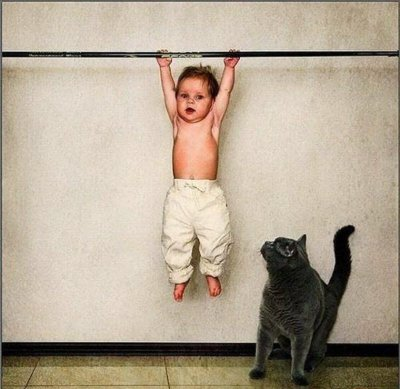
\includegraphics[width=0.8\textwidth]{babydoingpullups}
    \caption{How hard can it be if a baby can do it?}
    \label{fig::easy}
\end{figure}

If you need help, there is a lot of help topics in for form of online forums and wiki's. A google search of your formatting problems is a good start but here's a list of some resources to get started if you're new at \LaTeX:

\begin{itemize}
	\item \url{http://www.sharelatex.com} - Documentation and general help
    \item \url{http://www.overleaf.com} - Free online \LaTeX environment that has a word count function for the times when you're doing the bare minimum 
    \item \url{https://stackoverflow.com} - Answers to \LaTeX questions and all of your other homework questions. 
    \item \url{reu.dimacs.rutgers.edu/Symbols.pdf} - a cheat sheet for the math environment.
    \item \url{http://www.bibtex.org/} - Help for using \BibTeX. Mendeley, Zotero and a few other reference managers have \BibTeX support and can be linked easily. 
\end{itemize}


\endinput